\documentclass[runningheads]{llncs}

\usepackage[T1]{fontenc}
\usepackage[utf8]{inputenc}
\usepackage[numbers,sort&compress]{natbib}
\usepackage{url}
\usepackage{booktabs}
\usepackage{amsfonts}
\usepackage{amsmath}
\usepackage{amssymb}
\usepackage{nicefrac}
\usepackage{microtype}
\usepackage{xcolor}
\usepackage{multirow}
\usepackage{graphicx}
\graphicspath{{./}{../}}
\usepackage[hidelinks]{hyperref}

\begin{document}

\title{Expected Free Energy as Belief-Dependent Utility for $\rho$-POMDPs}

\titlerunning{EFE as Belief-Dependent Utility for $\rho$-POMDPs}

\author{Anonymous Author(s)}

\authorrunning{Anonymous Author(s)}

\institute{Anonymized for blind review}

\maketitle

\begin{abstract}
An agent acting under partial observability must decide when to gather information and which observations are worth their cost. Standard POMDPs value information only through its eventual effect on reward. The $\rho$-POMDP framework instead rewards uncertainty reduction directly through a belief-dependent utility $\rho$, but in practice both the choice of $\rho$ and the weight placed on it are tuned by hand for every task. We show that active inference supplies a derived relative coefficient in information units. Minimizing Expected Free Energy (EFE) is exactly equivalent to solving a $\rho$-POMDP whose utility is expected information gain at $w{=}1$. The identification is exact under log scoring rules \citep{bernardo1979}. Under a shared reward convention it is an empirically robust untuned default, not a scale-invariant automatic calibration. We prove this for observe-then-commit POMDPs and extend it to factored observation POMDPs covering interleaved observe-act settings. Across Tiger through RockSample to Structural Inspection with over $65{,}000$ states, untuned $w{=}1$ sits near the reward-maximizing Pareto knee and remains competitive with per-task tuned information bonuses.
\keywords{Active inference \and Expected free energy \and $\rho$-POMDPs \and Epistemic value \and Belief-dependent utility \and Partial observability \and Information gain}
\end{abstract}

\section{Introduction}

Decision-making under partial observability requires agents to balance exploiting current knowledge against gathering information to reduce uncertainty about hidden states. In standard POMDPs, information gathering has no intrinsic value. It is useful only insofar as it leads to higher expected reward. This creates a well-known difficulty: the exploration--exploitation trade-off must be resolved either by the planning horizon or by heuristic exploration bonuses.

The $\rho$-POMDP framework \citep{araya2010} addresses this by extending POMDPs with a belief-dependent utility $\rho(b)$ that allows the agent to derive value directly from properties of its belief state, enabling explicit optimization over uncertainty reduction or information gain alongside task reward. However, the choice of $\rho$ remains largely heuristic and environment-specific.

Separately, the Active Inference (AIF) framework \citep{friston2010, parr2019} casts perception and action as approximate Bayesian inference, selecting policies that minimize Expected Free Energy (EFE). EFE naturally decomposes into a pragmatic term (goal-seeking) and an epistemic term (information-seeking). Because both terms come from a single variational objective, their relative coefficient is fixed once pragmatic value is identified with task reward. In the discrete-state formulation we use, that coefficient is $w{=}1$ in information units (Proposition~\ref{prop:equivalence}). The claim is exact under log scoring rules \citep{bernardo1979} and, under a shared reward convention, an empirically robust untuned default. It is not scale-invariant.

We propose substituting EFE as $\rho$ in $\rho$-POMDPs, yielding an agent whose epistemic foraging is a consequence of its objective rather than an engineered bonus.\footnote{A full version with proofs, extended experiments, robustness analyses, and POMCP comparisons is available at \url{https://anonymous.4open.science/r/rho-aif}.} Our contributions are:
\begin{enumerate}
    \item A formal bridge between $\rho$-POMDPs and active inference (Proposition~\ref{prop:equivalence}) for observe-then-commit POMDPs, extended to factored observation POMDPs (Proposition~\ref{prop:factored}) covering interleaved settings where the hidden state is preserved by information-gathering actions, with a formal characterization of when $w{=}1$ is near-optimal (Proposition~\ref{prop:nearopt}).
    \item Controlled comparison against multiple baselines across six observe-then-commit environments and four RockSample instances, with Pareto analysis showing $w{=}1$ Pareto-dominates same-horizon planning on Diagnosis and Bandit, remaining competitive with tuned Planning+IG.
    \item Characterization of when EFE-as-$\rho$ helps. The advantage grows with state space size and observation action count, with large gains over reward-only planning on multi-observation benchmarks, though tuned Planning+IG can still lead on particular metrics.
\end{enumerate}

\section{Related Work}

\paragraph{POMDPs, $\rho$-POMDPs, and value of information.}
POMDPs formalize sequential decision-making under state uncertainty \citep{smallwood1973, kaelbling1998}. Online solvers such as POMCP \citep{silver2010} plan from the current belief using MCTS with UCB1, exploring implicitly through stochastic simulations rather than explicitly valuing information gain. \citet{araya2010} introduced $\rho$-POMDPs. When $\rho$ is convex the PWLC structure is preserved \citep{fehr2018, benchetrit2025}. POMDP-IR \citep{spaan2015} adds explicit information rewards. \citet{satsangi2018} note equivalence to $\rho$-POMDPs. \citet{bernardo1979} grounds information-as-utility under log scoring. \citet{walraven2024} connect AIF to POMDP information gathering. Common $\rho$ choices remain heuristic. We supply a derived information-unit weight under a shared reward convention. This paper includes an observe-then-commit IDS baseline (full version).

\paragraph{Active inference and EFE.}
The Active Inference (AIF) framework \citep{friston2010} casts perception and action as variational inference under the free-energy principle \citep{parr2022}. \citet{friston2015} formalized the decomposition of EFE into extrinsic (goal-seeking) and epistemic (information-seeking) components arising from a single variational bound \citep{dacosta2020, parr2019}, requiring no tunable exploration weight. The mathematical foundations have been examined critically \citep{millidge2021, champion2024, devries2025}. \citet{friston2021} introduced sophisticated inference, a recursive extension that \citet{dacosta2020b} proved recovers Bellman-optimal policies for any finite horizon. Our recursive EFE agent is derived from this framework, adapted to the $\rho$-POMDP commit-action structure. Intrinsic motivation methods \citep{schmidhuber1991, pathak2017, itti2009, bellemare2016, houthooft2016, burda2019} and control-as-inference approaches \citep{todorov2007, levine2018, haarnoja2018, millidge2020, sajid2021} all require tunable bonus weights. Our formalism fixes a derived information-unit weight under a shared reward convention. \citet{maisto2025} combined AIF with MCTS for large POMDPs. Our MCTS-EFE variant follows this direction.

\section{Methodology}
\label{sec:methodology}

\subsection{The $\rho$-POMDP framework}

We restrict attention to observe-then-commit $\rho$-POMDPs, in which the action set $\mathcal{A}$ partitions into observation actions $\mathcal{A}_\text{obs}$ (which update the belief at known cost but do not change the hidden state) and terminal commit actions $\mathcal{A}_\text{com}$ (which end the episode with state-dependent reward). A $\rho$-POMDP extends the standard POMDP with a belief-dependent utility $\rho : \Delta(S) \rightarrow \mathbb{R}$. The agent's objective becomes:
\begin{equation}
    \pi^* = \arg\max_\pi \mathbb{E}_\pi \left[ \sum_{t=0}^{H} \gamma^t \left( R(s_t, a_t) + \rho(b_t) \right) \right]
\end{equation}
When $\rho = 0$ we recover the standard POMDP. When $\rho$ encodes information gain, the agent is explicitly rewarded for reducing uncertainty.

\subsection{Expected Free Energy as $\rho$}

In the standard AIF formulation, the EFE for a policy $\pi$ at future time $\tau$ is:
\begin{equation}
    \mathcal{G}(\pi) = \underbrace{- \mathbb{E}_{Q(o_\tau|\pi)}[\ln P(o_\tau|C)]}_{\text{Pragmatic value}} - \underbrace{\mathbb{E}_{Q(o_\tau|\pi)}\left[D_{\mathrm{KL}}\left[Q(s_\tau|o_\tau, \pi) \,\|\, Q(s_\tau|\pi)\right]\right]}_{\text{Epistemic value}}
\end{equation}
where $P(o_\tau|C)$ encodes preferred outcomes and $D_{\mathrm{KL}}$ measures expected information gain. In our observe-then-commit setting, the pragmatic term reduces to expected reward for commit actions and known observation cost for observation actions. The epistemic term is the expected information gain $I_k(b) = H(b) - \mathbb{E}_o[H(b'_o \mid \text{obs}_k)]$.

Following the sophisticated inference scheme of \citet{friston2021}, the EFE agent evaluates actions via a recursive tree search over belief states:
\begin{equation}
    \mathcal{G}(\text{observe}_k) = c_k - I_k(b) + \mathbb{E}_{o}\!\left[\min_a \mathcal{G}(a \mid b'_o)\right]
    \label{eq:efe_recursive}
\end{equation}
The agent selects $\arg\min_a \mathcal{G}(a)$. Our deterministic $\arg\min$ corresponds to precision $\beta \to \infty$, eliminating an additional tunable knob. When EFE is written in nats, expected information gain enters on the same footing as the variational KL terms, which is why the $\rho$-POMDP reduction carries $w{=}1$ exactly (Proposition~\ref{prop:equivalence}).

\subsection{Formal equivalence with $\rho$-POMDPs}
\label{subsec:formal_rho_equiv}

We generalize the standard $\rho$-POMDP formulation to action-dependent belief utilities $\rho(b, a)$, where the augmented reward becomes $R(s,a) + \rho(b,a)$. Define $V(a, b, d) \triangleq -\mathcal{G}(a, b, d)$. Then Equation~\ref{eq:efe_recursive} becomes:
\begin{align}
    V(\text{observe}_k, b, d) &= -c_k + I_k(b) + \mathbb{E}_o\!\left[\max_a V(a, b'_o, d{+}1)\right] \label{eq:bellman_obs} \\
    V(\text{commit}_i, b, d) &= \mathbb{E}_b[R_i] \label{eq:bellman_commit}
\end{align}
This is exactly the Bellman recursion for a $\rho$-POMDP with action-dependent belief utility:

\begin{proposition}
\label{prop:equivalence}
Define $\rho_{\mathrm{EFE}}(b, a) = I_a(b)$ if $a$ is an observation action and $0$ if $a$ is a commit action, where $I_a(b) = H(b) - \mathbb{E}_{o|a}[H(b'_o)]$. Then for undiscounted finite horizon ($\gamma{=}1$), minimizing recursive EFE (Eq.~\ref{eq:efe_recursive}) over horizon $H$ produces the same policy as solving the $\rho$-POMDP Bellman equation $V^*(b) = \max_a \{R(b,a) + \rho_{\mathrm{EFE}}(b,a) + \mathbb{E}_o[V^*(b'_o)]\}$ over the same horizon.
\end{proposition}
\begin{proof}[Proof sketch]
The negation $V = -\mathcal{G}$ converts $\arg\min \mathcal{G}$ to $\arg\max V$. For observation actions, $V = -c_k + I_k(b) + \mathbb{E}_o[\max_{a'} V(a', b'_o)]$, matching the $\rho$-POMDP Bellman backup with $R(b, \text{obs}_k) = -c_k$ and $\rho = I_k(b)$. For commit actions, $V = \mathbb{E}_b[R_i]$ with $\rho = 0$. The recursive structure is identical, so policies agree at every belief node.
\end{proof}

This equivalence is a notational bridge---a corollary of Bellman optimality for sophisticated inference \citep{dacosta2020b} specialized to $\rho = I_a(b)$. Identifying pragmatic value with task reward chooses $P(o|C) \propto \exp(\beta R)$ with $\beta{=}1$ per reward unit. Keeping $w$ fixed while rescaling rewards by $k$ rescales the effective weight by $1/k$, so $w{=}1$ is not scale-invariant. The claim is exact under log scoring \citep{bernardo1979} and, under a shared reward convention, a robust untuned default. The implementation uses bits. Nat/bit conversion rescales $w$ by $\ln 2 \approx 0.69$, within the Pareto knee.

\begin{proposition}
\label{prop:nearopt}
Consider a two-state observe-then-commit $\rho$-POMDP with uniform prior, observation accuracy $p > \tfrac{1}{2}$, cost $c > 0$, and commit rewards $R^+$, $R^- < 0$. Let $\alpha = |R^-|/R^+$ and $I_{\max} = \ln 2 - H_{\text{post}}(p)$. The lower observation threshold at $H{=}1$ is
\begin{equation*}
    w^*_{\mathrm{lo}} = \frac{c \;-\; \left(p - \tfrac{1}{2}\right)(1 + \alpha)\,R^+}{\,I_{\max}\,}.
\end{equation*}
At the post-first-observation belief $b{=}(p,1{-}p)$, the upper (over-observation) threshold is $w^*_{\mathrm{hi}} = (c - \mathrm{VoI}_2(b))/I(b)$ when $\mathrm{VoI}_2 < c$, else $0$. At $H{=}2$, $w \in (w^*_{\mathrm{lo}}, w^*_{\mathrm{hi}})$ is the near-optimality interval. Under the paper's reward convention, $w{=}1$ lies in this interval for Tiger, Diagnosis, and Tileworld.
\end{proposition}

Table~\ref{tab:alpha_eta} reports corrected thresholds (nats). Bandit omitted as multi-arm, so Prop.~\ref{prop:nearopt} does not apply directly. Testbed places $w{=}1$ near $w^*_{\mathrm{hi}} \approx 1.01$ (over-exploration). High-asymmetry environments have $w^*_{\mathrm{lo}} \ll 0$ and $w^*_{\mathrm{hi}} \approx 7$--$8$.

\begin{table}[ht]
\centering
\caption{Thresholds (nats) from Proposition~\ref{prop:nearopt}. Bandit omitted (multi-arm).}
\label{tab:alpha_eta}
\begin{small}
\begin{tabular}{lccccc}
\toprule
Env. & $\alpha$ & $\eta$ & $w^*_{\mathrm{lo}}$ & $w^*_{\mathrm{hi}}$ & $w^*_{\mathrm{ret}}$ \\
\midrule
Testbed & $1.0$ & $1.31$ & $-3.06$ & $1.01$ & $0.5$ \\
Tiger & $10.0$ & $0.27$ & $-138.66$ & $6.89$ & $1.0$ \\
Diagnosis & $5.0$ & $0.19$ & $-88.20$ & $7.91$ & $0.5$ \\
Tileworld & $5.0$ & $0.19$ & $-88.20$ & $7.91$ & $0.5$ \\
\bottomrule
\end{tabular}
\end{small}
\end{table}

\paragraph{Extension to factored observation POMDPs.}
\label{par:frontier}

\begin{definition}[Factored observation POMDP]
\label{def:factored}
A POMDP is a factored observation POMDP if its state decomposes as $s = (s_{\mathrm{vis}}, s_{\mathrm{hid}})$ and the action set partitions into: (i)~observation actions that produce observations about $s_{\mathrm{hid}}$ without changing it, (ii)~navigation actions that change $s_{\mathrm{vis}}$ without changing $s_{\mathrm{hid}}$, and (iii)~exploitation actions that yield reward dependent on $s_{\mathrm{hid}}$.
\end{definition}

RockSample \citep{smith2004} is an instance: $s_{\mathrm{vis}}$ is the agent's position, $s_{\mathrm{hid}}$ is the vector of rock qualities, check actions are observation actions, moves are navigation, and sample/exit are exploitation actions.

\begin{proposition}
\label{prop:factored}
In a factored observation POMDP (Definition~\ref{def:factored}), let $b$ denote the belief over $s_{\mathrm{hid}}$. For any action $a$ that preserves $s_{\mathrm{hid}}$, the transition--observation coupling term vanishes: $\Delta_T(b, a) = 0$, and $\rho_{\mathrm{EFE}}(b, a) = I_a(b)$ for observation actions, $\rho_{\mathrm{EFE}}(b, a) = 0$ for navigation actions.
\end{proposition}
\begin{proof}[Proof sketch]
When $a$ preserves $s_{\mathrm{hid}}$, the belief update depends only on the observation likelihood, identical to the observe-then-commit case. The posterior that would incorporate transitions coincides with the observation-only posterior, so $D_{\mathrm{KL}}[b'_{o,T} \| b'_o] = 0$, and the $\rho$-POMDP Bellman equation follows as in Proposition~\ref{prop:equivalence}.
\end{proof}

This covers RockSample, mobile sensor placement, and sequential testing with spatial access costs. The key requirement breaks when information-gathering itself alters the hidden state ($\Delta_T \neq 0$). We discuss this limitation in Section~\ref{sec:discussion}.

\subsection{Agents}

We compare six agents (Table~\ref{tab:agents}), all sharing the same belief-update machinery and differing only in objective function and planning depth.

\begin{table}[ht]
\centering
\caption{Agent specifications. All use exact Bayesian belief updates over a known generative model.}
\label{tab:agents}
\begin{small}
\begin{tabular}{lccl}
\toprule
Agent & $\rho$ function & Horizon & Controls for \\
\midrule
Myopic & $\rho = 0$ & $H{=}1$ & Weakest baseline \\
Planning & $\rho = 0$ & $H > 1$ & Planning depth \\
Info Gain & $w \cdot I(b)$ & $H{=}1$ & Epistemic bonus (myopic) \\
Planning+IG & $w \cdot I(b)$ & $H > 1$ & IG + planning depth \\
EFE & $I_a(b)$ via EFE & $H > 1$ & Joint objective (Prop.~\ref{prop:equivalence}) \\
Epistemic-only & $I_a(b)$ only & $H > 1$ & Ablation: no pragmatic term \\
\bottomrule
\end{tabular}
\end{small}
\end{table}

Planning+IG is the critical baseline: by Proposition~\ref{prop:equivalence}, EFE is exactly Planning+IG with $w{=}1$. Any advantage is attributable to the weight choice, not a different mechanism. For Info Gain and Planning+IG, $w$ is tuned per environment via grid search over $\{0.1, 0.5, 1, 2, 5, 10, 20, 50, 100\}$ on 200 tuning episodes.

\section{Experiments}

All environments are implemented as OpenAI Gymnasium environments following the observe-then-commit structure. Main results use 1{,}000 episodes per seed across 5 random seeds for a total of 5{,}000 episodes. Statistical comparisons use $t$-tests with Holm--Bonferroni correction.

\paragraph{Tiger} \citep{kaelbling1998}. Two states, one observation action (listen, accuracy 0.85), two commit actions. Rewards: correct $+10$, incorrect $-100$, listen cost $-1$.

\paragraph{Sequential diagnosis.} $N{=}4$ conditions, $K{=}2$ binary tests (accuracy 0.80), $N$ diagnose actions. Correct $+10$, incorrect $-50$, test cost $-1$. The agent must choose which test to run.

\paragraph{Structured bandit.} $K{=}4$ arms, $K$ inspect actions (accuracy 0.80, cost $-0.5$), $K$ pull actions. Best arm $+10$, others $+1$. The agent must choose which arm to inspect.

\paragraph{Tileworld.} An $N{\times}N$ grid ($N{=}6$, $|S|{=}36$) with a hidden target tile. $K{=}6$ scan actions partition the grid via bit-level splits of row/column indices (accuracy $0.80$, cost $-1$). $N^2$ commit actions collect at a specific cell (correct $+10$, incorrect $-50$). A spatial generalization of diagnosis (Figure~\ref{fig:tw_comparison}).

\paragraph{RockSample} \citep{smith2004}. An $N{\times}N$ grid with $K$ rocks at known positions, each with hidden binary quality. Move, check, sample, and exit actions form the interleaved observe-act structure addressed by Proposition~\ref{prop:factored}. We evaluate RS[5,3], RS[7,4], RS[7,8], and RS[11,11].

\paragraph{Structural inspection.} $N$ components at known spatial locations, each with a hidden binary state (nominal/faulty, prior $p_{\text{fault}}{=}0.3$). Two non-destructive test types: visual (accuracy $0.70$, cost $-0.5$) and detailed (accuracy $0.90$, cost $-2$). Asymmetric penalties: missed fault $-50$, false alarm $-5$. Tests do not change fault states, so this is a factored observation POMDP. We evaluate $N{=}8$ ($|S|{=}256$) and $N{=}16$ ($|S|{=}65{,}536$).

\section{Results}

\subsection{Core environments}

\begin{table}[ht]
\centering
\caption{Results across three core environments (5{,}000 total episodes: 1{,}000 per seed $\times$ 5 seeds). $w^*$: per-environment tuned weight. Reward shown as mean $\pm$ SE.}
\label{tab:main}
\begin{small}
\begin{tabular}{llccc}
\toprule
Environment & Agent & Obs. & Success & Reward \\
\midrule
\multirow{4}{*}{\shortstack[l]{Tiger\\[-1pt]{\scriptsize $H{=}6,\;w^*{=}20$}}} & Myopic & $1.00$ & 84.6\% & $-7.98 \pm 0.56$ \\
& Planning & $4.28$ & 99.5\% & $+5.15 \pm 0.12$ \\
& Planning+IG & $4.20$ & 99.4\% & $+5.19 \pm 0.12$ \\
& \textbf{EFE} & $\mathbf{4.22}$ & $\mathbf{99.5\%}$ & $\mathbf{+5.23 \pm 0.11}$ \\
\midrule
\multirow{4}{*}{\shortstack[l]{Diagnosis\\[-1pt]{\scriptsize $H{=}3,\;w^*{=}100$}}} & Myopic & $2.00$ & 64.2\% & $-13.48 \pm 0.41$ \\
& Planning & $5.91$ & 89.2\% & $-2.37 \pm 0.26$ \\
& Planning+IG & $13.21$ & 99.3\% & $-3.63 \pm 0.10$ \\
& \textbf{EFE} & $\mathbf{9.70}$ & $\mathbf{97.0\%}$ & $\mathbf{-1.52 \pm 0.16}$ \\
\midrule
\multirow{4}{*}{\shortstack[l]{Bandit\\[-1pt]{\scriptsize $H{=}2,\;w^*{=}100$}}} & Myopic & $2.04$ & 61.7\% & $+5.53 \pm 0.06$ \\
& Planning & $3.24$ & 69.6\% & $+5.65 \pm 0.06$ \\
& Planning+IG & $12.41$ & 99.8\% & $+3.78 \pm 0.04$ \\
& \textbf{EFE} & $\mathbf{5.16}$ & $\mathbf{87.3\%}$ & $\mathbf{+6.27 \pm 0.05}$ \\
\bottomrule
\end{tabular}
\end{small}
\end{table}

On Tiger (single observation action), all multi-step agents achieve ${\sim}99.5\%$ success. EFE matches tuned alternatives without weight selection. The Epistemic-only ablation commits at chance on all environments, proving the pragmatic term is essential. Pure information gain without reward alignment produces catastrophic exploration.

On Diagnosis and Bandit, EFE Pareto-dominates same-horizon Planning with higher success and better reward without weight search (Diagnosis: $97.0\%$ vs.\ $89.2\%$, reward $-1.52$ vs.\ $-2.37$. Bandit: $87.3\%$ vs.\ $69.6\%$, $+6.27$ vs.\ $+5.65$). Success-tuned Planning+IG ($w{=}100$) reaches near-ceiling success at substantial reward cost from over-exploration. EFE is the competitive untuned trade-off. Headline comparisons include tuned Planning+IG, not only $w{=}0$. In the success--reward plane (Figure~\ref{fig:pareto}), EFE sits at the Pareto knee.

\subsection{Pareto analysis: the information-unit weight $w{=}1$}
\label{sec:pareto}

By Proposition~\ref{prop:equivalence}, EFE is exactly Planning+IG with $w{=}1$. We sweep $w$ from $0.01$ to $200$ on all environments (Figure~\ref{fig:pareto}).

\begin{figure}[t]
\centering
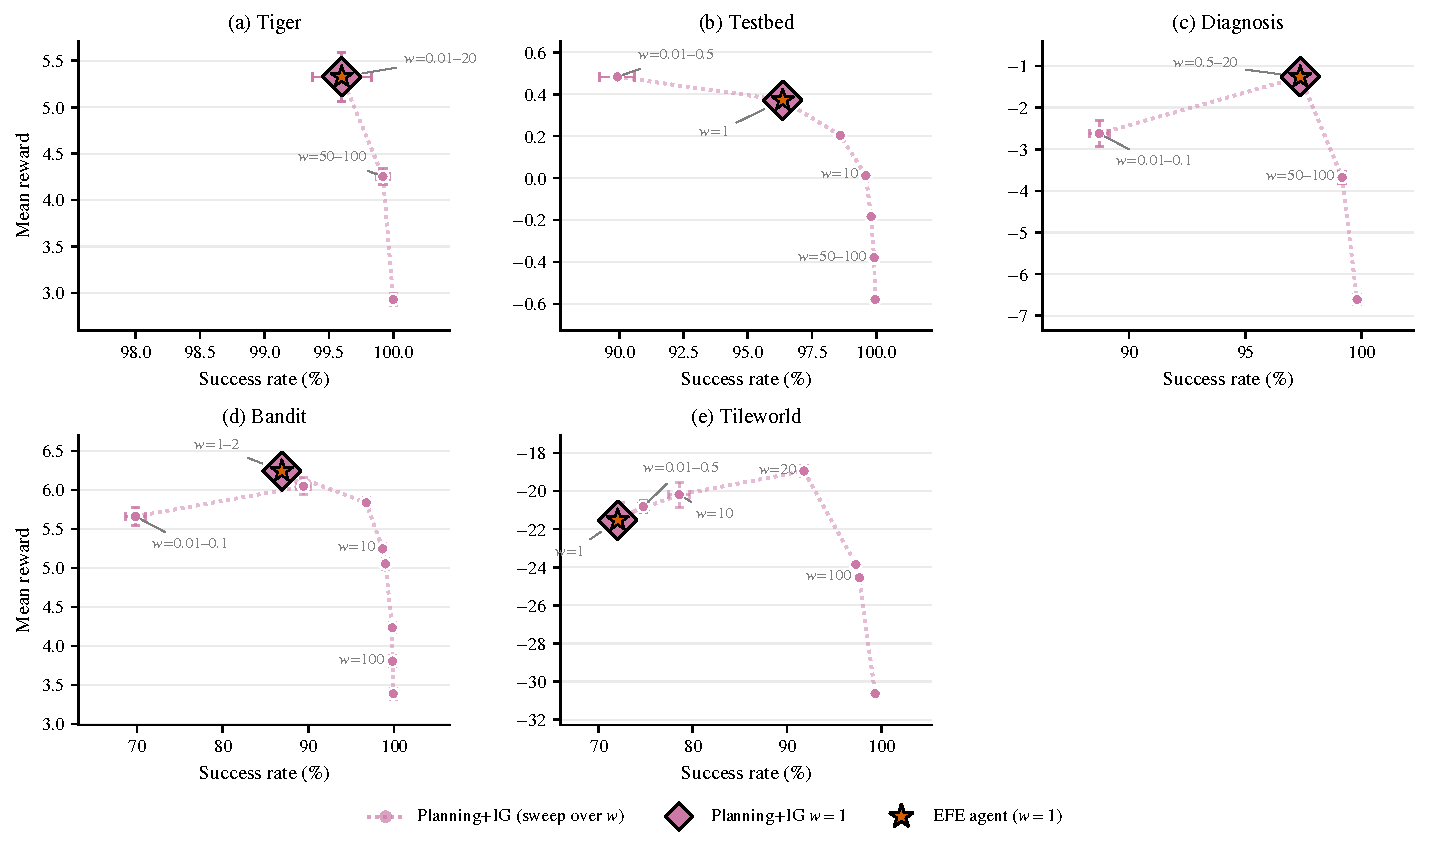
\includegraphics[width=\linewidth]{figures/fig_pareto.pdf}
\caption{Pareto analysis: success rate vs.\ mean reward as $w$ varies from 0.01 to 200. Diamond: Planning+IG at $w{=}1$. Star: EFE agent. By Proposition~\ref{prop:equivalence} with shared deterministic tie-breaking, the markers coincide. Both sit at or near the Pareto knee, where further weight increases buy marginal accuracy at substantial reward cost.}
\label{fig:pareto}
\end{figure}

On every environment, $w{=}1$ sits near the reward-maximizing weight $w^*_{\text{ret}}$, while the success-maximizing weight $w^*_{\text{succ}}$ lies at $20$--$200$. The contribution of EFE is deriving a principled weight from the variational bound that is near-optimal for reward maximization, rather than a grid search whose optimum changes by orders of magnitude across tasks.

\subsection{Tileworld: spatial epistemic foraging}
\label{sec:tileworld}

\begin{table}[ht]
\centering
\caption{Tileworld $6{\times}6$ (2{,}500 episodes: 500 per seed $\times$ 5 seeds, $H{=}2$). Tuned weight $w^*{=}100$.}
\label{tab:tileworld}
\begin{small}
\begin{tabular}{lccc}
\toprule
Agent & Scans & Success & Reward \\
\midrule
Myopic & $0.00$ & 2.7\% & $-48.39$ \\
Planning ($H{=}2$) & $15.68$ & 73.7\% & $-21.47$ \\
Planning+IG ($w{=}100$) & $33.38$ & 98.4\% & $-24.31$ \\
\textbf{EFE} ($H{=}2$) & $\mathbf{14.81}$ & $\mathbf{72.8\%}$ & $\mathbf{-21.13}$ \\
\bottomrule
\end{tabular}
\end{small}
\end{table}

EFE achieves the highest reward ($-21.13$), scanning 14.81 times, less than half of Planning+IG's 33.38 scans, which erode reward despite reaching 98.4\% success. Figure~\ref{fig:tw_comparison} visualizes the mechanism: EFE concentrates belief efficiently via partition-based narrowing and commits once confident, while Planning lacks scan-selection guidance and Info Gain continues scanning past the point of diminishing returns.

\begin{figure}[t]
\centering
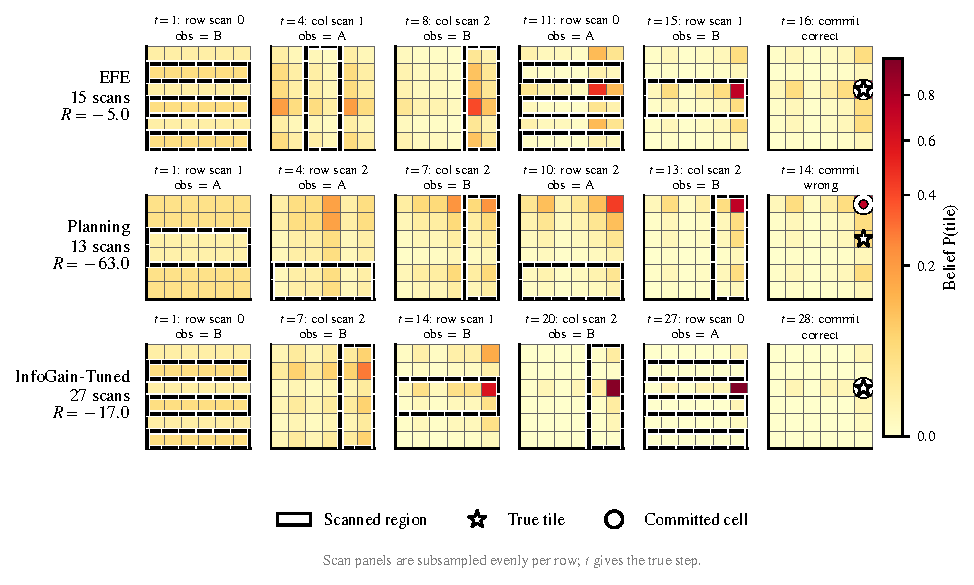
\includegraphics[width=\linewidth]{figures/fig_tileworld_comparison.pdf}
\caption{Agent comparison on the same $6{\times}6$ Tileworld episode. EFE (top) commits correctly with efficient scanning. Planning (middle) commits with less directed exploration. Info Gain (bottom) over-scans past the point of diminishing returns. Red circle: committed cell. Green star: target.}
\label{fig:tw_comparison}
\end{figure}

\paragraph{Spatial scaling.} We scale the grid from $4{\times}4$ to $8{\times}8$ with all agents (Figure~\ref{fig:tw_scaling}). At $8{\times}8$ ($|S|{=}64$), reward-only Planning collapses to $2.5\%$ success while EFE maintains $66.5\%$. EFE ($w{=}1$) achieves the best reward at every scale. The $w^*_{\text{ret}}$ does not shift with $|S|$ (EFE's reward remains highest), but the gap between $w^*_{\text{ret}}$ and $w^*_{\text{succ}}$ widens, so safety-critical applications at large scale would benefit from higher weights.

\begin{figure}[t]
\centering
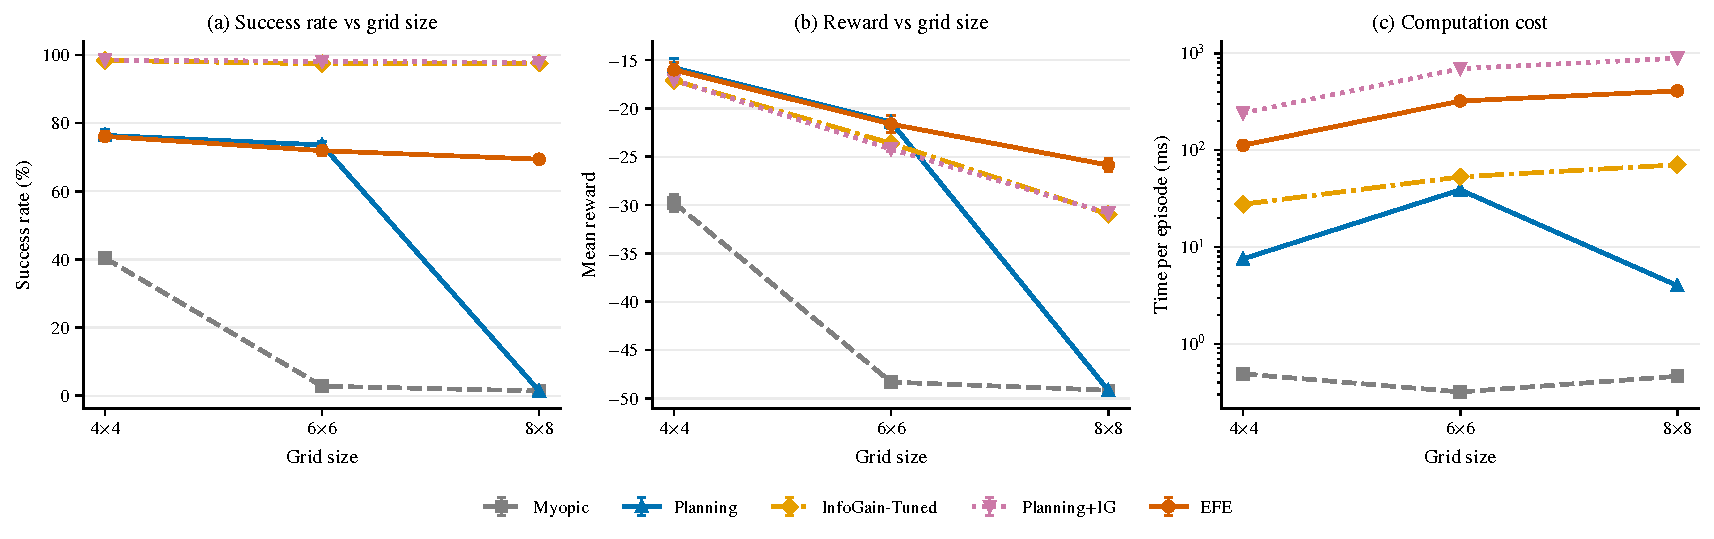
\includegraphics[width=\linewidth]{figures/fig_tileworld_scaling.pdf}
\caption{Tileworld scaling ($H{=}2$, 200 episodes per seed $\times$ 5 seeds). Planning collapses at $8{\times}8$ ($|S|{=}64$). EFE maintains $66.5\%$. Tuned Planning+IG ($w{=}100$) achieves $98.0\%$ but at higher reward cost.}
\label{fig:tw_scaling}
\end{figure}

\subsection{Interleaved observe-act: RockSample}
\label{sec:rocksample}

\begin{table}[ht]
\centering
\caption{RockSample results (500 episodes $\times$ 5 seeds for RS[5,3]--[7,8] and 50 $\times$ 2 seeds for RS[11,11]). EFE ($w{=}1$) achieves the highest or near-highest reward on all instances while avoiding bad rocks, confirming Proposition~\ref{prop:factored}.}
\label{tab:rocksample}
\begin{small}
\begin{tabular}{llccccc}
\toprule
Instance & Agent & Steps & Checks & Good & Bad & Reward \\
\midrule
\multirow{4}{*}{RS[5,3]} & Greedy & -- & -- & $1.49$ & $1.51$ & $+3.71$ \\
& Planning ($w{=}0$) & -- & -- & $1.06$ & $0.08$ & $+14.00$ \\
& Planning+IG ($w{=}5$) & -- & -- & $1.34$ & $0.02$ & $\mathbf{+15.67}$ \\
& EFE ($w{=}1$) & -- & -- & $1.34$ & $0.02$ & $\mathbf{+15.67}$ \\
\midrule
\multirow{4}{*}{RS[7,4]} & Greedy & -- & -- & $1.98$ & $2.02$ & $-0.88$ \\
& Planning ($w{=}0$) & -- & -- & $0.98$ & $0.04$ & $+14.39$ \\
& Planning+IG ($w{=}5$) & -- & -- & $1.50$ & $0.02$ & $+13.47$ \\
& EFE ($w{=}1$) & -- & -- & $1.38$ & $0.00$ & $\mathbf{+15.47}$ \\
\midrule
\multirow{4}{*}{RS[7,8]} & Greedy & -- & -- & $3.50$ & $4.50$ & $-7.09$ \\
& Planning ($w{=}0$) & -- & -- & $0.45$ & $0.05$ & $+11.75$ \\
& Planning+IG ($w{=}5$) & -- & -- & $2.55$ & $0.05$ & $\mathbf{+20.82}$ \\
& EFE ($w{=}1$) & -- & -- & $2.15$ & $0.05$ & $+19.57$ \\
\midrule
\multirow{4}{*}{\shortstack[l]{RS[11,11]\\[-1pt]{\scriptsize $|S|{=}2048$}}} & Greedy & -- & -- & $5.33$ & $5.67$ & $-21.90$ \\
& Planning ($w{=}0$) & -- & -- & $0.50$ & $0.01$ & $+13.64$ \\
& Planning+IG ($w{=}5$) & -- & -- & $0.53$ & $0.01$ & $\mathbf{+13.66}$ \\
& EFE ($w{=}1$) & -- & -- & $0.50$ & $0.01$ & $+13.64$ \\
\bottomrule
\end{tabular}
\end{small}
\end{table}

On RS[5,3], EFE ties Planning+IG. On RS[7,4], EFE leads. On RS[7,8], Planning+IG ($w{=}5$) beats EFE on reward ($+20.82$ vs.\ $+19.57$), both far above Planning ($+11.75$). Greedy samples without checking. On RS[11,11], informed agents are nearly tied at shallow depth.

\subsection{Structural inspection}
\label{sec:inspection}

\begin{table}[ht]
\centering
\caption{Structural Inspection results. $N{=}8$: 2{,}500 episodes. $N{=}16$: 1{,}000 episodes. Reward: mean $\pm$ SE. Greedy diagnoses without testing. Bold: best accuracy/reward (not always EFE). Accuracy: fraction correctly diagnosed.}
\label{tab:inspection}
\begin{small}
\begin{tabular}{llccccc}
\toprule
Instance & Agent & Accuracy & Missed & Tests & Reward \\
\midrule
\multirow{4}{*}{\shortstack[l]{$N{=}8$\\[-1pt]{\scriptsize $|S|{=}256$}}} & Greedy & 70.7\% & $2.34$ & $0.0$ & $-114.33 \pm 1.33$ \\
& Planning ($w{=}0$) & 73.0\% & $0.07$ & $12.7$ & $\mathbf{-17.85 \pm 0.34}$ \\
& Planning+IG ($w{=}5$) & $\mathbf{94.9\%}$ & $0.10$ & $18.7$ & $-22.82 \pm 0.35$ \\
& EFE ($w{=}1$) & $87.9\%$ & $0.08$ & $18.0$ & $-20.60 \pm 0.34$ \\
\midrule
\multirow{4}{*}{\shortstack[l]{$N{=}16$\\[-1pt]{\scriptsize $|S|{=}65{,}536$}}} & Greedy & 70.0\% & $4.81$ & $0.0$ & $-237.46 \pm 2.93$ \\
& Planning ($w{=}0$) & 78.2\% & $0.26$ & $22.3$ & $-46.09 \pm 0.94$ \\
& Planning+IG ($w{=}5$) & $\mathbf{91.4\%}$ & $0.24$ & $28.1$ & $\mathbf{-43.51 \pm 0.85}$ \\
& EFE ($w{=}1$) & $86.1\%$ & $0.27$ & $32.8$ & $-45.71 \pm 0.94$ \\
\bottomrule
\end{tabular}
\end{small}
\end{table}

EFE is a competitive untuned trade-off, not uniquely best. On $N{=}8$, Planning wins reward. On $N{=}16$, Planning+IG wins accuracy and reward. EFE still beats Planning by $+7.9$pp accuracy at comparable reward. High asymmetry ($\alpha = 25$) places $w{=}1$ in the Prop.~\ref{prop:nearopt} near-optimality regime.

\subsection{Summary}

Taken together, the experiments tell a consistent story. EFE matches Planning+IG at $w{=}1$, confirming Propositions~\ref{prop:equivalence} and~\ref{prop:factored}, and that information-unit weight lands at the Pareto knee without per-environment search. On Diagnosis and Bandit, untuned EFE Pareto-dominates same-horizon planning. Across Tileworld, RockSample, and Inspection, the advantage over $w{=}0$ Planning grows with state space size and observation count, up to $|S|{=}65{,}536$.

\section{Discussion}
\label{sec:discussion}

\paragraph{When does EFE-as-$\rho$ help?}
EFE's advantage requires two conditions: (1)~multiple observation actions with differential informativeness, and (2)~sufficient planning horizon for recursive EFE to propagate epistemic value. When (1) fails (Tiger), reward-only planning matches EFE. As the state space grows, the reward signal becomes too diffuse to guide scan selection and EFE's advantage increases (Figure~\ref{fig:tw_scaling}). EFE is most effective when reward asymmetry $\alpha \geq 5$, multiple explicit observation actions exist, state spaces satisfy $|S| \geq 16$, hidden states are preserved under observation and navigation (factored POMDPs), and the weight cannot be tuned per-task. EFE is not recommended when $\alpha \approx 1$, in navigation-style POMDPs where observations are a side effect of translation, or under heavy discounting ($\gamma < 0.99$). Discounting truncates the effective planning horizon below the number of observations needed for disambiguation, erasing EFE's advantage.

\paragraph{The information-unit weight and near-optimality.}
EFE supplies a derived relative coefficient in information units under a fixed reward convention---not a scale-free automatic calibration. The Pareto analysis (Figure~\ref{fig:pareto}) shows $w{=}1$ sits near $w^*_{\text{ret}}$, while success-maximizing $w^*_{\text{succ}}$ (main-table Planning+IG) lies at $20$--$200$. Success-tuned weights transfer poorly across environments (extended version). Under a shared reward convention, $w{=}1$ is a robust untuned default. High-asymmetry settings place $w{=}1$ interior to $(w^*_{\mathrm{lo}}, w^*_{\mathrm{hi}})$.
\paragraph{Limitations.}
The formal equivalence holds for factored observation POMDPs but not for settings where information-gathering changes the hidden state (destructive testing, adversarial surveillance). The EFE agent assumes a known generative model. Robustness experiments in the extended version show graceful degradation up to $\pm 0.15$ accuracy mismatch, with EFE's epistemic drive providing a partial buffer against overconfident models. The exact tree search cost $\mathcal{O}(K \cdot |\mathcal{O}|^H)$ limits practical horizons to $H{=}2$--$3$. An MCTS-EFE variant using EFE as a leaf heuristic achieves $97.2\%$ success at $H{=}10$ on Tiger with 500 simulations, outperforming POMCP ($89.7\%$) at matched compute (extended version). Extending the formal treatment to slowly drifting hidden states and to full model learning (where AIF and BAMDPs converge) remains future work. This work is primarily theoretical, though the principled derivation of exploration weights could benefit safety-critical decision-making by reducing reliance on ad-hoc tuning.

\section{Conclusion}

The $\rho$-POMDP framework and active inference converge on a belief-dependent utility adding information gain at $w{=}1$---a derived relative coefficient in information units, exact under log scoring \citep{bernardo1979}, empirically robust under a shared reward convention, and not scale-invariant. Tuned Planning+IG can exceed EFE on some metrics. EFE remains the competitive untuned default. Proposition~\ref{prop:factored} carries the bridge to factored observation POMDPs, from RockSample through Structural Inspection with over $65{,}000$ states.

\begin{credits}
\subsubsection{\ackname} Removed for anonymous submission.

\subsubsection{\discintname}
The authors have no competing interests to declare that are relevant to the content of this article.
\end{credits}

% Bibliography (LNCS/CCIS numbered style)
\begin{thebibliography}{38}

\bibitem[Araya-L\'{o}pez et~al.(2010)]{araya2010}
M.~Araya-L\'{o}pez, O.~Buffet, V.~Thomas, and F.~Charpillet.
\newblock A {POMDP} extension with belief-dependent rewards.
\newblock In \emph{Advances in Neural Information Processing Systems}, 2010.

\bibitem[Bellemare et~al.(2016)]{bellemare2016}
M.~Bellemare, S.~Srinivasan, G.~Ostrovski, T.~Schaul, D.~Saxton, and R.~Munos.
\newblock Unifying count-based exploration and intrinsic motivation.
\newblock In \emph{Advances in Neural Information Processing Systems}, 2016.

\bibitem[Bernardo(1979)]{bernardo1979}
J.~M. Bernardo.
\newblock Expected information as expected utility.
\newblock \emph{The Annals of Statistics}, 7(3):686--690, 1979.

\bibitem[Benchetrit et~al.(2025)]{benchetrit2025}
R.~Benchetrit, I.~Lev-Yehudi, A.~Zhitnikov, and V.~Indelman.
\newblock Anytime incremental $\rho${POMDP} planning in continuous spaces.
\newblock \emph{arXiv preprint arXiv:2502.02549}, 2025.

\bibitem[Burda et~al.(2019)]{burda2019}
Y.~Burda, H.~Edwards, A.~Storkey, and O.~Klimov.
\newblock Exploration by random network distillation.
\newblock In \emph{International Conference on Learning Representations}, 2019.

\bibitem[Champion et~al.(2026)]{champion2024}
T.~Champion, H.~Bowman, D.~Markovi\'{c}, and M.~Grze\'{s}.
\newblock Reframing the expected free energy: Four formulations and a unification.
\newblock \emph{Neural Computation}, 38(3):439--469, 2026.

\bibitem[Da~Costa et~al.(2020)]{dacosta2020}
L.~Da~Costa, T.~Parr, N.~Sajid, S.~Veselic, V.~Neacsu, and K.~Friston.
\newblock Active inference on discrete state-spaces: A synthesis.
\newblock \emph{Journal of Mathematical Psychology}, 99:102447, 2020.

\bibitem[Da~Costa et~al.(2023)]{dacosta2020b}
L.~Da~Costa, N.~Sajid, T.~Parr, K.~Friston, and R.~Smith.
\newblock Reward maximization through discrete active inference.
\newblock \emph{Neural Computation}, 35(5):807--852, 2023.

\bibitem[de~Vries et~al.(2025)]{devries2025}
B.~de~Vries, W.~Nuijten, T.~van~de~Laar, et~al.
\newblock Expected free energy-based planning as variational inference.
\newblock \emph{arXiv preprint arXiv:2504.14898}, 2025.

\bibitem[Fehr et~al.(2018)]{fehr2018}
M.~Fehr, O.~Buffet, V.~Thomas, and J.~Dibangoye.
\newblock $\rho$-{POMDP}s have {L}ipschitz-continuous $\epsilon$-optimal value functions.
\newblock In \emph{Advances in Neural Information Processing Systems}, 2018.

\bibitem[Friston(2010)]{friston2010}
K.~Friston.
\newblock The free-energy principle: a unified brain theory?
\newblock \emph{Nature Reviews Neuroscience}, 11(2):127--138, 2010.

\bibitem[Friston et~al.(2015)]{friston2015}
K.~Friston, F.~Rigoli, D.~Ognibene, C.~Mathys, T.~FitzGerald, and G.~Pezzulo.
\newblock Active inference and epistemic value.
\newblock \emph{Cognitive Neuroscience}, 6(4):187--214, 2015.

\bibitem[Friston et~al.(2021)]{friston2021}
K.~Friston, L.~Da~Costa, D.~Hafner, C.~Hesp, and T.~Parr.
\newblock Sophisticated inference.
\newblock \emph{Neural Computation}, 33(3):713--763, 2021.

\bibitem[Haarnoja et~al.(2018)]{haarnoja2018}
T.~Haarnoja, A.~Zhou, P.~Abbeel, and S.~Levine.
\newblock Soft actor-critic: Off-policy maximum entropy deep reinforcement learning with a stochastic actor.
\newblock In \emph{International Conference on Machine Learning}, 2018.

\bibitem[Heins et~al.(2022)]{heins2022}
C.~Heins, B.~Millidge, D.~Demekas, B.~Klein, K.~Friston, I.~Couzin, and A.~Tschantz.
\newblock pymdp: A {P}ython library for active inference in discrete state spaces.
\newblock \emph{Journal of Open Source Software}, 7(73):4098, 2022.

\bibitem[Houthooft et~al.(2016)]{houthooft2016}
R.~Houthooft, X.~Chen, Y.~Duan, J.~Schulman, F.~De~Turck, and P.~Abbeel.
\newblock {VIME}: Variational information maximizing exploration.
\newblock In \emph{Advances in Neural Information Processing Systems}, 2016.

\bibitem[Howard(1966)]{howard1966}
R.~A. Howard.
\newblock Information value theory.
\newblock \emph{IEEE Transactions on Systems Science and Cybernetics}, 2(1):22--26, 1966.

\bibitem[Itti and Baldi(2009)]{itti2009}
L.~Itti and P.~Baldi.
\newblock {B}ayesian surprise attracts human attention.
\newblock \emph{Vision Research}, 49(10):1295--1306, 2009.

\bibitem[Kaelbling et~al.(1998)]{kaelbling1998}
L.~P. Kaelbling, M.~L. Littman, and A.~R. Cassandra.
\newblock Planning and acting in partially observable stochastic domains.
\newblock \emph{Artificial Intelligence}, 101(1--2):99--134, 1998.

\bibitem[Levine(2018)]{levine2018}
S.~Levine.
\newblock Reinforcement learning and control as probabilistic inference: Tutorial and review.
\newblock \emph{arXiv preprint arXiv:1805.00909}, 2018.

\bibitem[Lindley(1956)]{lindley1956}
D.~V. Lindley.
\newblock On a measure of the information provided by an experiment.
\newblock \emph{The Annals of Mathematical Statistics}, 27(4):986--1005, 1956.

\bibitem[Maisto et~al.(2025)]{maisto2025}
D.~Maisto, F.~Gregoretti, K.~J. Friston, and G.~Pezzulo.
\newblock Active inference tree search in large {POMDP}s.
\newblock \emph{Neurocomputing}, 623:129319, 2025.

\bibitem[Millidge et~al.(2020)]{millidge2020}
B.~Millidge, A.~Tschantz, A.~K. Seth, and C.~L. Buckley.
\newblock On the relationship between active inference and control as inference.
\newblock In \emph{International Workshop on Active Inference}, pp.\ 3--11. Springer, 2020.

\bibitem[Millidge et~al.(2021)]{millidge2021}
B.~Millidge, A.~Tschantz, and C.~L. Buckley.
\newblock Whence the expected free energy?
\newblock \emph{Neural Computation}, 33(2):447--482, 2021.

\bibitem[Oudeyer and Kaplan(2007)]{oudeyer2007}
P.-Y. Oudeyer and F.~Kaplan.
\newblock What is intrinsic motivation? {A} typology of computational approaches.
\newblock \emph{Frontiers in Neurorobotics}, 1:6, 2007.

\bibitem[Parr and Friston(2019)]{parr2019}
T.~Parr and K.~J. Friston.
\newblock Generalised free energy and active inference.
\newblock \emph{Biological Cybernetics}, 113(5):495--513, 2019.

\bibitem[Parr et~al.(2022)]{parr2022}
T.~Parr, G.~Pezzulo, and K.~J. Friston.
\newblock \emph{Active Inference: The Free Energy Principle in Mind, Brain, and Behavior}.
\newblock MIT Press, 2022.

\bibitem[Pathak et~al.(2017)]{pathak2017}
D.~Pathak, P.~Agrawal, A.~A. Efros, and T.~Darrell.
\newblock Curiosity-driven exploration by self-supervised prediction.
\newblock In \emph{International Conference on Machine Learning}, 2017.

\bibitem[Sajid et~al.(2021)]{sajid2021}
N.~Sajid, P.~J. Ball, T.~Parr, and K.~J. Friston.
\newblock Active inference: Demystified and compared.
\newblock \emph{Neural Computation}, 33(3):674--712, 2021.

\bibitem[Satsangi et~al.(2018)]{satsangi2018}
Y.~Satsangi, S.~Whiteson, F.~A. Oliehoek, and M.~T.~J. Spaan.
\newblock Exploiting submodular value functions for scaling up active perception.
\newblock \emph{Autonomous Robots}, 42(2):209--233, 2018.

\bibitem[Schmidhuber(1991)]{schmidhuber1991}
J.~Schmidhuber.
\newblock A possibility for implementing curiosity and boredom in model-building neural controllers.
\newblock In \emph{Proc.\ International Conference on Simulation of Adaptive Behavior}, pp.\ 222--227, 1991.

\bibitem[Silver and Veness(2010)]{silver2010}
D.~Silver and J.~Veness.
\newblock {Monte-Carlo} planning in large {POMDP}s.
\newblock In \emph{Advances in Neural Information Processing Systems}, 2010.

\bibitem[Smallwood and Sondik(1973)]{smallwood1973}
R.~D. Smallwood and E.~J. Sondik.
\newblock The optimal control of partially observable {M}arkov processes over a finite horizon.
\newblock \emph{Operations Research}, 21(5):1071--1088, 1973.

\bibitem[Smith and Simmons(2004)]{smith2004}
T.~Smith and R.~Simmons.
\newblock Heuristic search value iteration for {POMDP}s.
\newblock In \emph{Uncertainty in Artificial Intelligence}, 2004.

\bibitem[Spaan et~al.(2015)]{spaan2015}
M.~T.~J. Spaan, T.~S. Veiga, and P.~U. Lima.
\newblock Decision-theoretic planning under uncertainty with information rewards for active cooperative perception.
\newblock \emph{Autonomous Agents and Multi-Agent Systems}, 29(6):1157--1185, 2015.

\bibitem[Todorov(2006)]{todorov2007}
E.~Todorov.
\newblock Linearly-solvable {M}arkov decision problems.
\newblock In \emph{Advances in Neural Information Processing Systems}, 2006.

\bibitem[Tschantz et~al.(2020)]{tschantz2020}
A.~Tschantz, B.~Millidge, A.~K. Seth, and C.~L. Buckley.
\newblock Reinforcement learning through active inference.
\newblock In \emph{ICLR Workshop on Bridging AI and Cognitive Science}, 2020.

\bibitem[Walraven et~al.(2025)]{walraven2024}
E.~Walraven, J.~Sijs, and G.~Burghouts.
\newblock Information gathering in {POMDP}s using active inference.
\newblock \emph{Autonomous Agents and Multi-Agent Systems}, 39(1):3, 2025.

\end{thebibliography}

\end{document}
